\documentclass[10pt,a4paper]{article}
\usepackage[UTF8,fontset = windows]{ctex}
\setCJKmainfont[BoldFont=黑体,ItalicFont=楷体]{华文中宋}
\usepackage{amssymb,amsmath,amsfonts,amsthm,mathrsfs,dsfont,graphicx}
\usepackage{ifthen,indentfirst,enumerate,color,titletoc}
\usepackage{tikz}
\usepackage{makecell}
\usepackage{longtable}
\usetikzlibrary{arrows,calc,intersections,patterns}
\usepackage[bf,small,indentafter,pagestyles]{titlesec}
\usepackage[top=1in, bottom=1in,left=0.8in,right=0.8in]{geometry}
\renewcommand{\baselinestretch}{1.65}
\newtheorem{defi}{定义~}
\newtheorem{eg}{例~}
\newtheorem{ex}{~}
\newtheorem{rem}{注~}
\newtheorem{thm}{定理~}
\newtheorem{coro}{推论~}
\newtheorem{axiom}{公理~}
\newtheorem{prop}{性质~}
\newcommand{\blank}[1]{\underline{\hbox to #1pt{}}}
\newcommand{\bracket}[1]{(\hbox to #1pt{})}
\newcommand{\onech}[4]{\par\begin{tabular}{p{.9\textwidth}}
A.~#1\\
B.~#2\\
C.~#3\\
D.~#4
\end{tabular}}
\newcommand{\twoch}[4]{\par\begin{tabular}{p{.46\textwidth}p{.46\textwidth}}
A.~#1& B.~#2\\
C.~#3& D.~#4
\end{tabular}}
\newcommand{\vartwoch}[4]{\par\begin{tabular}{p{.46\textwidth}p{.46\textwidth}}
(1)~#1& (2)~#2\\
(3)~#3& (4)~#4
\end{tabular}}
\newcommand{\fourch}[4]{\par\begin{tabular}{p{.23\textwidth}p{.23\textwidth}p{.23\textwidth}p{.23\textwidth}}
A.~#1 &B.~#2& C.~#3& D.~#4
\end{tabular}}
\newcommand{\varfourch}[4]{\par\begin{tabular}{p{.23\textwidth}p{.23\textwidth}p{.23\textwidth}p{.23\textwidth}}
(1)~#1 &(2)~#2& (3)~#3& (4)~#4
\end{tabular}}
\begin{document}
\begin{enumerate}[1.]


%1_21

\item 已知全集$U=\{x|x<2\}$, 集合$A=\{x|x<1\}$, 则$\complement_UA=$\blank{50}.
\item 设集合$A=\{x||x-2|<1, \ x\in\mathbf{R}\}$, $B=\{x|\dfrac{x-3}{x-1}\ge 0\}$, 则$A\cup B=$\blank{50}.
\item 若函数$f(x)=2^x-3$, 则$f^{-1}(1)=$\blank{50}.
\item 设函数$f(x)=\begin{cases} 2^{-x}-1,  & x\le 0,\\ x^\frac 12, & x>0,\end{cases}$ 若$f(x_0)>1$, 则$x_0$的取值范围是\blank{50}.
\item 已知$x\in (0,\dfrac{\pi}2)$, 则方程$\begin{vmatrix} 2\sin x   & 1  \\1  & 2\cos x  \end{vmatrix}=0$的解集是\blank{50}.
\item 关于$x$的不等式$^2+ax+1>0$有解, 则实数$a$的取值范围是\blank{50}.
\item 已知$f(x)=x^2+2(a-2)x+4$, 对$x\in[-3, 1]$, $f(x)>0$恒成立, 则实数$a$的取值范围是\blank{50}.
\item 设正数$a,b$, 当$(a+b)^2+\dfrac{1}{4ab}$取最小值时, $a$的值为\blank{50}.
\item 设椭圆$\Gamma:\dfrac{x^2}{a^2}+{y^2}=1$($a>1$)的左顶点为$A$, 过点$A$的直线$l$与$\Gamma$相交于另一点$B$, 与$y$轴相交于点$C$. 若$|OA|=|OC|$, $|AB|=|BC|$, 则$a=$\blank{50}.
\item 已知常数$b,c\in \mathbf{R}$. 若函数$f(x)=(x^2+x-2)(x^2+bx+c)$为偶函数, 则$b+c=$\blank{50}.
\item 记$a,b,c,d,e,f$为$1,2,3,4,5,6$的任意一个排列, 则使得$(a+b)(c+d)(e+f)$为奇数的排列共有\blank{50}个.
\item 已知函数$f(x)=|x+\dfrac 1x+a|$, 若对任意实数$a$, 关于$x$的不等式$f(x)\ge m$在区间$[\dfrac 12,3]$上总有解, 则实数$m$的取值范围为\blank{50}.
\item 已知$x\in\mathbf{R}$, 则"$x>0$"是"$x>1$"的\bracket{20}.
\fourch{充分非必要条件}{必要非充分条件}{充要条件}{既非充分又非必要条件}
\item 已知$a,b,c$是互不相等的正数, 则下列不等式中正确的是\bracket{20}.
\twoch{$|a-b|<|a-c|+|c-b|$}{$a^2+\dfrac{1}{a^2}\le a+\dfrac{1}{a}$}{$|a-b|+\dfrac{1}{a-b}\ge 2$}{$\sqrt{a+3}-\sqrt{a+1}\le\sqrt{a+2}-\sqrt a$}
\item 设$a,b,c$表示三条互不重合的直线, $\alpha,\beta$表示两个不重合的平面, 则使得``$a\parallel b$''成立	的一个充分条件为\bracket{20}.
\twoch{$a\perp c$, $b\perp c$}{$a\parallel \alpha$, $b\parallel \alpha$}{$a\parallel \alpha$, $a\parallel \beta$, $\alpha \cap \beta =b$}{$b\perp \alpha$, $c\parallel \alpha$, $a\perp c$}
\item 已知函数$y=f(x)$的定义域为$(0,+\infty)$, 满足对任意$x\in (0,+\infty)$, 恒有$f[f(x)-\dfrac 1x]=4$. 若函数$y=f(x)-4$的零点个数为有限的$n$($n\in \mathbf{N}^*$)个, 则$n$的最大值为\bracket{20}.
\fourch{$1$}{$2$}{$3$}{$4$}
\item 如图, 在长方体$ABCD-A_1B_1C_1D_1$中, $2AB=BC=AA_1$, 点$M$为棱$C_1D_1$上的动点.
\begin{center}
    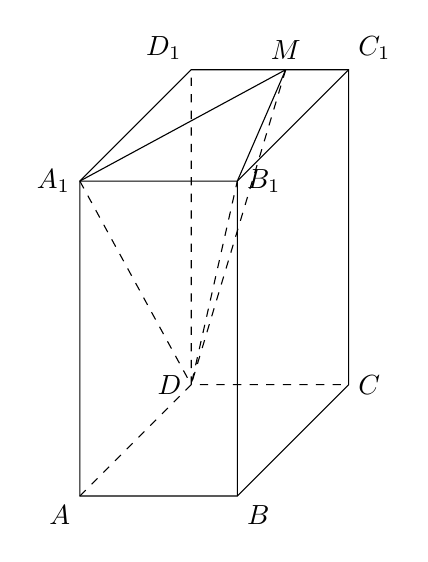
\begin{tikzpicture}
        \draw (0,0) node [below left] {$A$} coordinate (A) --++ (2,0) node [below right] {$B$} coordinate (B) --++ (45:{4/2}) node [right] {$C$} coordinate (C)
        --++ (0,4) node [above right] {$C_1$} coordinate (C1)
        --++ (-2,0) node [above left] {$D_1$} coordinate (D1) --++ (225:{4/2}) node [left] {$A_1$} coordinate (A1) -- cycle;
        \draw (A) ++ (2,4) node [right] {$B_1$} coordinate (B1) -- (B) (B1) --++ (45:{4/2}) (B1) --++ (-2,0);
        \draw [dashed] (A) --++ (45:{4/2}) node [left] {$D$} coordinate (D) --++ (2,0) (D) --++ (0,4);
        \draw ($(D1)!0.6!(C1)$) node [above] {$M$} coordinate (M) (M) -- (A1) (M) -- (B1);
        \draw [dashed] (M) -- (D) -- (B1) (A1) -- (D);
    \end{tikzpicture}
\end{center}
(1) 求三棱锥$D-A_1B_1M$与长方体$ABCD-A_1B_1C_1D_1$的体积比;\\
(2) 若$M$为棱$C_1D_1$的中点, 求直线$DB_1$与平面$DA_1M$所成角的大小.
\item 已知常数$a\in \mathbf{R}^+$, 函数$f(x)=3^x+a^2\cdot 3^{-x}$.\\
(1) 若$a=\sqrt 3$, 解关于$x$的不等式$f(x)<4$;\\
(2) 若$f(x)$在$[3,+\infty)$上为增函数, 求$a$的取值范围.
\item 某居民小区为缓解业主停车难的问题, 拟对小区内一块扇形空地$AOB$进行改建. 如图所示, 平行四边形$OMPN$区域为停车场, 其余部分建成绿地, 点$P$在围墙$\overset\frown{AB}$上, 点$M$和$N$分别在道路$OA$和道路$OB$上, 且$OA=60\text{m}$, $\angle AOB=\dfrac\pi 3$. 设$\angle POB=\theta$.
\begin{center}
    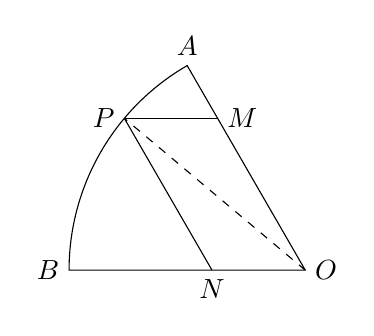
\begin{tikzpicture}
        \draw (0,0) node [left] {$B$} arc (180:140:3) node [left] {$P$} coordinate (P) arc (140:120:3) node [above] {$A$} -- (3,0) node [right] {$O$}-- cycle;
        \draw [dashed] (3,0) -- (P);
        \draw (P) --++ ({3/sin(60)*sin(20)},0) node [right] {$M$};
        \draw (P) --++ (-60:{3/sin(60)*sin(40)}) node [below] {$N$};
    \end{tikzpicture}
\end{center}
(1) 求停车场面积$S$(单位: $\text{m}^2$)关于$\theta$的函数关系式, 并写出$\theta$的取值范围;\\
(2) 求停车场面积$S$的最大值以及相应$\theta$的值.
\item 在平面直角坐标系$xOy$中, 抛物线$\Gamma:y^2=4x$, 点$C(1,0)$. $A,B$为$\Gamma$上的两点, $A$在第一象限, 满足$\overrightarrow{OA}\cdot \overrightarrow{OB}=-4$.\\
(1) 求证: 直线$AB$过定点, 并求定点坐标;\\
(2) 设$P$为$\Gamma$上的动点, 求$\dfrac{|OP|}{|CP|}$的取值范围;\\
(3) 记$\triangle AOB$的面积为$S_1$, $\triangle BOC$的面积为$S_2$, 求$S_1+S_2$的最小值.
\item 已知函数$f(x)=x|x-a|$, 其中$a$为常数.\\
(1) 当$a=1$时, 解不等式$f(x)<2$;\\
(2) 已知$g(x)$是以$2$为周期的偶函数, 且当$0\le x\le 1$时, 有$g(x)=f(x)$. 若$a<0$, 且$g(\dfrac 32)=\dfrac 54$, 求函数$y=g(x)$($x\in [1,2]$)的反函数;\\
(3) 若在$[0,2]$上存在$n$个不同的点$x_i$($i=1,2,\cdots,n$, $n\ge 3$), $x_1<x_2<\cdots <x_n$, 使得$|f(x_1)-f(x_2)|+|f(x_2)-f(x_3)|+\cdots+|f(x_{n-1})-f(x_n)|=8$, 求实数$a$的取值范围.

%2_14

\item 设集合$A=\{1,2,3\}$, $B=\{x|x<3\}$, 则$A\cap B=$\blank{50}.
\item 已知常数$a\in \mathbf{R}$, 函数$f(x)=x^2$($-1\le x\le a$)是偶函数, 则$a=$\blank{50}.
\item 设函数$f(x)=\lg (x+1)$的反函数为$f^{-1}(x)$, 则$f^{-1}(1)=$\blank{50}.
\item 函数$f(x)=\sqrt{\dfrac{1-x}x}$的定义域为\blank{50}.
\item 已知常数$a\in \mathbf{R}$, 设$p:1\le x<2$, $q:x<a$. 若$p$是$q$的充分条件, 则$a$的取值范围为\blank{50}.
\item 关于$x$的方程$\log_2 x+\log_2(x-3)=2$的解为\blank{50}.
\item 已知函数$f(x)$的定义域为$\mathbf{R}$, 满足对任意$x\in \mathbf{R}$, 恒有$f(x)+f(x+2)=4$. 若$f(1)+f(2)=1$, 则$f(2021)-f(2020)=$\blank{50}.
\item 已知常数$a\in \mathbf{R}$, 函数$f(x)=a\cdot 4^x+2^x+1$在$[3,+\infty)$上单调递减, 则$a$的取值范围为\blank{50}.
\item 已知常数$m,n\in \mathbf{Z}$, 若对任意$x\in [0,+\infty)$, 不等式$(mx-2)(x^2-2n)\ge 0$恒成立, 则$m+n$的取值集合为\blank{50}.
\item 已知常数$a\in \mathbf{R}$, 函数$f(x)=x^2-4x+a$, $g(x)=ax^2-8x+4$. 若存在$x_0\in (0,+\infty)$, 使得$f(x_0)$与$g(x_0)$都不是正数, 则$a$的取值范围为\blank{50}.
\item 对任意的非零实数$a,b$, 下列不等式恒成立的是\bracket{20}.
\twoch{$\dfrac ba+\dfrac ab\ge 2$}{$(a+b)(\dfrac 1a+\dfrac 1b)\ge 4$}{$\dfrac{|a+b|}2\ge 2\sqrt{|ab|}$}{$\dfrac{a^2+b^2}{2}\ge (\dfrac{a+b}2)^2$}
\item 设函数$f(x)$的定义域为$\mathbf{R}$, $f(x)$满足对任意$x_1,x_2\in \mathbf{R}$, 当$x_1\ne x_2$时, 恒有$|f(x_1)-f(x_2)|>2|x_1-x_2|$. 对于命题: \textcircled{1} $f(x)$的解析式可以是$f(x)=x^3+2021x$; \textcircled{2} $f(x)$的解析式可以是$f(x)=2021^{-x}$, 下列判断正确的是\bracket{20}.
\twoch{\textcircled{1}、\textcircled{2}均为真命题}{\textcircled{1}、\textcircled{2}均为假命题}{\textcircled{1}为真命题、\textcircled{2}为假命题}{\textcircled{1}为假命题、\textcircled{2}为真命题}
\item 已知常数$a\in \mathbf{R}$, 函数$f(x)=ax^2+\lg \dfrac{1+x}{1-x}$.\\
(1) 若$a=0$, 判断$f(x)$的单调性并证明;\\
(2) 问: 是否存在$a$, 使得$f(x)$为奇函数? 若存在, 求出所有$a$的值; 若不存在, 说明理由.
\item 设函数$f(x)$的定义域为$(0,+\infty)$, 若对任意$x\in (0,+\infty)$, 恒有$f(2x)=2f(x)$, 则称$f(x)$为``$2$阶缩放函数''.\\
(1) 已知函数$f(x)$为``$2$阶缩放函数'', 当$x\in (1,2]$时, $f(x)=1-\log_2 x$, 求$f(2\sqrt{2})$的值;\\
(2) 已知函数$f(x)$为``$2$阶缩放函数'', 当$x\in (1,2]$时, $f(x)=\sqrt{2x-x^2}$, 求证: 函数$y=f(x)-x$在$(1,+\infty)$上无零点.

%3_21
\item 设全集$U=\mathbf{R}$, $A=(-\infty ,3)$, 则$\complement_UA=$\blank{50}.	
\item 函数$f(x)=x^{- \frac 12}$的定义域为\blank{50}.
\item 已知函数$f(x)$的反函数$f^{-1}(x)=\log_2x$, 则$f(-1)=$\blank{50}.
\item 已知球的半径为$2$, 则它的体积为\blank{50}.	
\item 已知$\sin \alpha =-\dfrac{\sqrt 5}5$, $\alpha \in (-\dfrac{\pi}2,\dfrac{\pi}2)$ , 则$\sin (\alpha +\dfrac{3\pi}2)=$\blank{50}.
\item 已知圆锥的底面半径为$1\text{cm}$, 侧面积为$2\pi\text{cm}^2$, 则母线与底面所成角的大小为\blank{50}.
\item 已知$(x^2+\dfrac 2x)^n$的二项展开式中, 所有二项式系数的和为$512$, 则展开式中的常数项为\blank{50}(结果用数值表示).	
\item $f(x)$是偶函数, 当$x\ge 0$时, $f(x)=2^x-1$, 则不等式$f(x)>1$的解集为\blank{50}.
\item 方程$1+\log_2x=\log_2(x^2-3)$的解为\blank{50}.	
\item 已知函数$f(x)=\begin{cases}  x^2+(4a-3)x+3a,& x<0, \\ \log_a(x+1)+1,& x\ge 0, \end{cases}$($a>0$, $a\ne 1$)在$\mathbf{R}$上单调递减, 且关于$x$的方程$|f(x)|=2-x$恰好有两个不相等的实数解, 则$a$的取值范围是\blank{50}.
\item 我国古代数学名著《九章算术》中记载了有关特殊几何体的定义: 阳马指底面为矩形, 一侧棱垂直于底面的四棱锥, 堑堵指底面是直角三角形, 且侧棱垂直于底面的三棱柱. 某堑堵$ABC-A_1B_1C_1$, $AC\perp BC$, 若$A_1A=AB=2$, 当阳马$B-AA_1C_1C$的体积最大时, 二面角$C-A_1B-C_1$的大小为\blank{50}.
\begin{center}
    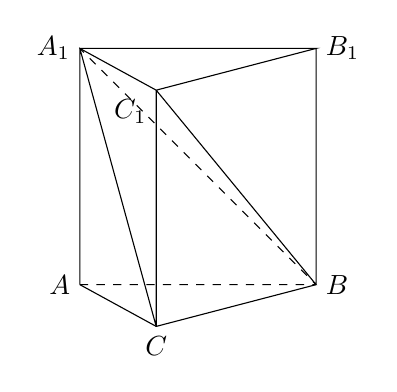
\begin{tikzpicture}[scale = 1.5]
        \draw (-1,0) node [left] {$A$} coordinate (A) -- (225:0.5) node [below] {$C$} coordinate (C) -- (1,0) node [right] {$B$} coordinate (B);
        \draw (A) --++ (0,2) node [left] {$A_1$} coordinate (A1) (B) --++ (0,2) node [right] {$B_1$} coordinate (B1) (C) --++ (0,2) node [below left] {$C_1$} coordinate (C1) (A1) -- (B1) -- (C1) -- (A1) -- (C) (C1) -- (B);
        \draw [dashed] (A) -- (B) -- (A1);
    \end{tikzpicture}
\end{center}
\item 对于全集$\mathbf{R}$的子集$A$, 定义函数$f_A(x)=\begin{cases}
1, &  x\in A,  \\0, & x\in \complement_{\mathbf{R}}A  \end{cases}$为$A$的特征函数, 设$A,B$为全集$\mathbf{R}$的子集,\\
\textcircled{1} 若$A\subseteq B$, 则$f_A(x)\le f_B(x)$; \textcircled{2} $f_{\complement_{\mathbf{R}}A}(x)=1-f_A(x)$;\\
\textcircled{3} ${f_{A\cap B}}(x)=f_A(x)\cdot f_B(x)$; \textcircled{4} $f_{A\cup B}(x)=f_A(x)+f_B(x)$;\\ \textcircled{5} $f_{A\cap \complement_\mathbf{R}B}(x)=f_A(x)-f_B(x)$; \textcircled{6} 对于任意$x\in \mathbf{R}$, 若$f_A(x)\cdot f_B(x)=0$恒成立, 则$A\cap B=\varnothing$.\\
其中正确的命题为\blank{50}(填所有正确命题的序号).
\item 已知实数$a,b$满足$a>b$, 则下列不等式中恒成立的是\bracket{20}。
\fourch{$a^2>b^2$}{$\dfrac 1a<\dfrac 1b$}{$|a|>|b|$}{$2^a>2^b$}
\item 下列函数中, 值域为$(0,+\infty)$的是\bracket{20}.
\fourch{$y=x^2$}{$y=\dfrac 2x$}{$y=2^x$}{$y=|\log_2x|$}
\item 从正方体的$8$个顶点中选取$4$个作为顶点, 可得到四面体的个数为\bracket{20}.
\fourch{$\mathrm{C}_8^4-12$}{$\mathrm{C}_8^4-8$}{$\mathrm{C}_8^4-6$}{$\mathrm{C}_8^4-4$}
\item 设集合$A=\{y|y=a^x,\ x>0\}$(其中常数$a>0,  \ a\ne 1$), $B=\{y|y=x^k,\ x\in A\}$(其中常数$k\in \mathbf{Q}$), 则``$k<0$''是``$A\cap B=\varnothing$''的\bracket{20}.
\twoch{充分非必要条件}{必要非充分条件}{充分必要条件}{既非充分又非必要条件}
\item 如图所示, 在直三棱柱$ABC-A_1B_1C_1$中, 底面是等腰直角三角形, $\angle ACB=90^\circ$, $CA=CB=CC_1=2$. 点$D,D_1$分别是棱$AC,A_1C_1$的中点.
\begin{center}
    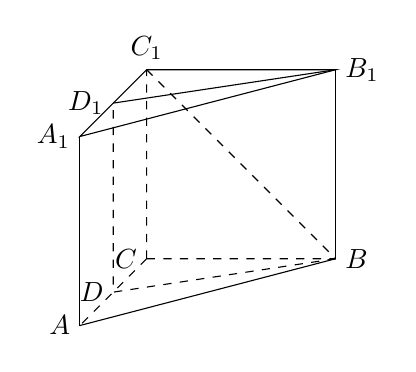
\begin{tikzpicture}[scale = 1.2]
        \draw [dashed] (0,0) node [left] {$C$} coordinate (C) -- (2,0) node [right] {$B$} coordinate (B) (C) -- (0,2) node [above] {$C_1$} coordinate (C1) (C) -- (225:1) node [left] {$A$} coordinate (A);
        \draw (A) --++ (0,2) node [left] {$A_1$} coordinate (A1) (B) --++ (0,2) node [right] {$B_1$} coordinate (B1);
        \draw (A) -- (B) (A1) -- (B1) -- (C1) -- cycle;
        \draw ($(A)!0.5!(C)$) node [left] {$D$} coordinate (D) ++ (0,2) node [left] {$D_1$} coordinate (D1);
        \draw (B1) -- (D1);
        \draw [dashed] (B) -- (D) -- (D1) (C1) -- (B);
    \end{tikzpicture}
\end{center}
(1)	求四棱锥$C-AA_1B_1B$的体积;\\
(2)	求直线$BC_1$与平面$DBB_1D_1$所成角的大小.
\item 设常数$k\in \mathbf{R}$, $f(x)=k\cos^2x+\sqrt 3\sin x\cos x$, $x\in \mathbf{R}$.\\
(1) 若$\tan \alpha =2$且$f(\alpha)=\sqrt 3$, 求实数$k$的值;\\
(2) 设$k=1$, $\triangle ABC$中, 内角$A,B,C$的对边分别为$a,b,c$. 若$f(A)=1$, $a=\sqrt 7$, $b=3$, 求$\triangle ABC$的面积$S$.
\item 东西向的铁路上有两个道口$AB$, 铁路两侧的公路分布如图, $C$位于$A$的南偏西$15^\circ$, 且位于$B$的南偏东$15^\circ$方向, $D$位于$A$的正北方向, $AC=AD=2km$, $C$处一辆救护车欲通过道口前往$D$处的医院送病人, 发现北偏东$45^\circ$方向的$E$处(火车头位置)有一列火车自东向西驶来, 若火车通过每个道口都需要$1$分钟, 救护车和火车的速度均为$60\text{km/h}$.
\begin{center}
    \begin{tikzpicture}[>=latex]
        \draw (-2,0) -- (2,0) (0,0) node [above right] {$A$} -- (0,2) node [right] {$D$};
        \draw (0,0) --++ (-105:2) node [below] {$C$} coordinate (C) --++ (105:2) node [above left] {$B$} -- (0,2); 
        \draw ({sqrt(2)},0) node [above] {$E$} -- (C);
        \draw [->] (-2,1) --++ (0.5,0) node [right] {东};
        \draw [->] (-2,1) --++ (0,0.5) node [above] {北};
    \end{tikzpicture}
\end{center}
(1) 判断救护车通过道口$A$是否会受火车影响, 并说明理由;\\
(2) 为了尽快将病人送到医院, 救护车应选择$AB$中的哪个道口? 通过计算说明.
\item 已知函数$f(x)=\dfrac{ax^2+1}{bx+c}$是奇函数, $a,b,c$为常数.\\
(1)	求实数$c$的值;\\
(2)	若$a,b\in \mathbf{Z}$, 且$f(1)=2$, $f(2)<3$, 求$f(x)$的解析式;\\
(3) 已知$b>0$, 若$f(x)\ge f(1)$在$(0,+\infty)$上恒成立, 且$\{x|f[f(x)]\ge x\}\cap [1,2]\ne \varnothing$, 求$b$的取值范围.
\item 记函数$f(x)$的定义域为$D$. 如果存在实数$a$、$b$使得$f(a-x)+f(a+x)=b$对任意满足$a-x\in D$且$a+x\in D$的$x$恒成立, 则称$f(x)$为$\Psi$函数.\\
(1) 设函数$f(x)=\dfrac 1x-1$, 试判断$f(x)$是否为$\Psi$函数, 若是求出$a,b$, 若不是请说明理由;\\
(2) 设函数$g(x)=\dfrac 1{2^x+t}$, 其中常数$t\ne 0$, 证明: $g(x)$是$\Psi$函数;\\
(3) 若$h(x)$是定义在$\mathbf{R}$上的$\Psi$函数, 且函数$h(x)$的图像关于直线$x=m$($m$为常数)对称, 试判断$h(x)$是否为周期函数? 并证明你的结论.

%4_16

\end{enumerate}
\end{document}